\section{Analysis}
In the analysis section we will be analyzing the 
errors resulting from the heuristic algorithm, discussing applications for the solutions 
provided to the Minimum Height Problem and discussing open problems regarding the Minimum Height Problem.

\subsection{Analysis of Errors}
Depending on the permutation, it is not always the case that making $\pi_{2}$ as 
zig-zaggy as possible results in a ladder with minimal height. Given the 
permutation $(2,4,5,3,1)$, \newline {\sc PreProcessRowOne(2,4,5,3,1)} returns $\pi_{2}=(2,4,3,5,1)$.
However,\newline$\pi_{2}=(2,4,3,5,1)$ does not lead to a 
ladder with  minimal height. Rather, the $\pi_{2}$ which leads 
to a ladder with minimal height is $(2,4,5,3,1)$. Notice 
how  $(2,4,5,3,1)$ is less zig-zaggy than $(2,4,3,5,1)$. 
To see the ladder resulting from the {\sc HeuristicAlgorithm} 
in comparison to the truly shortest ladder for the 
permutation $(2,4,5,3,1)$ please refer to Figure~\ref{Fig:ff}.\par 
\begin{figure}[ht]
    \centering 
    \begin{minipage}{.4\textwidth}
        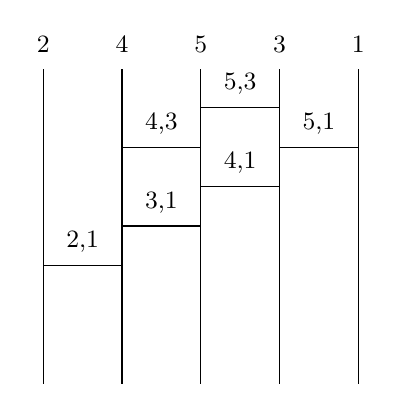
\begin{tikzpicture}
                
            \draw(0, 0) to (0, 4);
            \node at(0, 4.3){\small{$2$}};
            \draw(1, 0) to (1, 4);
            \node at(1, 4.3){\small{$4$}};
            \draw(2, 0) to (2, 4);
            \node at(2, 4.3){\small{$5$}};
            \draw(3, 0) to (3, 4);
            \node at(3, 4.3){\small{$3$}};
            \draw(4, 0) to (4, 4);
            \node at(4, 4.3){\small{$1$}};

            %%bars 
            \node at(2.5, 3.8)(a){\small{5,3}};
            \draw(2, 3.5) to (3, 3.5);

            \node at(1.5, 3.3)(a){\small{4,3}};
            \draw(1, 3) to (2, 3);

            \node at(3.5, 3.3)(a){\small{5,1}};
            \draw(3, 3) to (4, 3);

            \node at(2.5, 2.8)(a){\small{4,1}};
            \draw(2, 2.5) to (3, 2.5);


            \node at(1.5, 2.3)(a){\small{3,1}};
            \draw(1, 2) to (2, 2);

            \node at(.5, 1.8)(a){\small{2,1}};
            \draw(0, 1.5) to (1, 1.5);
        \end{tikzpicture}

    \end{minipage}
      \begin{minipage}{.4\textwidth}
        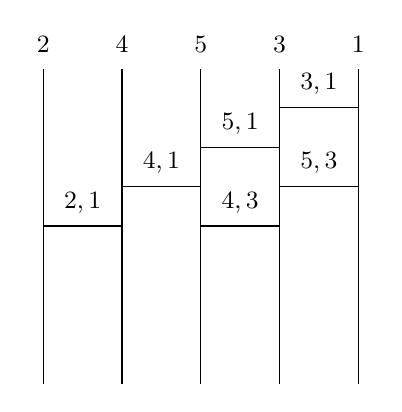
\begin{tikzpicture}
                
            \draw(0, 0) to (0, 4);
            \node at(0, 4.3){\small{$2$}};
            \draw(1, 0) to (1, 4);
            \node at(1, 4.3){\small{$4$}};
            \draw(2, 0) to (2, 4);
            \node at(2, 4.3){\small{$5$}};
            \draw(3, 0) to (3, 4);
            \node at(3, 4.3){\small{$3$}};
            \draw(4, 0) to (4, 4);
            \node at(4, 4.3){\small{$1$}};

            %%bars 
            \draw(3, 3.5) to (4, 3.5);\node at(3.5, 3.8){\small{$3,1$}};

            \draw(2, 3) to (3, 3);\node at(2.5, 3.3){\small{$5,1$}};
            \draw(1, 2.5) to (2, 2.5);\node at(1.5, 2.8){\small{$4,1$}};
            \draw(3, 2.5) to (4, 2.5);\node at(3.5, 2.8){\small{$5,3$}};
            \draw(0, 2) to (1, 2);\node at(.5, 2.3){\small{$2,1$}};
            \draw(2, 2) to (3, 2);\node at(2.5, 2.3){\small{$4,3$}};
        \end{tikzpicture}

    \end{minipage}

    
    \caption{{\sc HeuristicAlgorithm} ladder on the left, shortest ladder is on the right.}
    
    \label{Fig:ff}
    
\end{figure}

The assumption behind the {\sc HeuristicAlgorithm} is that the more bars that are 
inserted into a given row, the shorter the ladder will be. Thus, the {\sc HeuristicAlgorithm} is 
a greedy algorithm. Given a 
current row in the ladder, continue to insert as many bars into that row as possible.
Once done, move to the next row. However, the greedy approach only leads 
to a locally optimal solution; each row is locally optimized given the current state 
of $\pi_{k}$. This does not necessarily lead to a globally optimal insofar as 
the resulting ladder may not be a $MinL(\pi)$. To see a table containing ladders from the {\sc HeuristicAlgorithm}
in comparison to the ladders created by brute force please refer to Figure~\ref{Fig:MinLadders} in the appendix.

\subsection{Open Problems Related to the Minimum Height Problem}
\begin{itemize}
    \item Is there a deterministic and efficient algorithm for creating $MinL(\pi)$ given some arbitrary $\pi$?
\end{itemize}
\subsection{Applications}
The {\sc HeuristicAlgorithm} can be applied to other problems of compression. Most notable is creating the 
shortest $InvPi(\pi)$. Still thinking of what to add here. Not sure what this problem can be applied to.
